\IEEEraisesectionheading{\section{Introduction}\label{sec:introduction}}



\IEEEPARstart {3}{D} printing, or additive manufacturing, has drawn growing interests from researchers in computer graphics. Fused deposition modeling (FDM), stereolithographic (SLA), Selective Laser Melting (SLM) and Selective Laser Sintering (SLS) are the four most popular means of 3D printing techniques. Although 3D printing has seen its applications in producing arbitrarily intricate 3D models, the price of the printing materials, especially for those with high quality, are still outrageously high. Therefore, it is desirable to reduce materials used in the fabrication process. Note that this is also a critical operation for reducing production time and thus the total production cost. For this purpose, an efficient method is to minimize the support structures, which are removed in the post-processing phase of the fabrication task.

Autodesk MeshMixer provides a semiautomatic orientation optimization tool to minimize support volume, support area, structural strength, or a combination of these three attributes. However, it requires professional experience in setting the geometric parameters manually. A number of literatures have studied various factors that influence the volume of supports, e.g., optimizing the topology of the support structure \cite{DumasHL14,VanekGB14}, determining an optimal fabrication direction \cite{Zhang:2015,HildebrandBA13,padhye2011multi}, partitioning any given model into a set of separate parts that satisfy particular geometric properties such as being pyramidical \cite{Hu_siga14}, has minimal packing volume \cite{VanekGBMCSM14} or being inter-lockable \cite{SongFLF15}.


%However, the partition results of these methods do not simultaneously respect the geometric properties and the support-free printability of the portioned parts \youyi{vague, what are the geometry properties? the pyramid paper considers both?}. Further,


{\color{blue}{Although there exists some algorithms for partitioning models in an (almost) support-free fashion \cite{Hu_siga14}, no existing methods ever consider the problem of partitioning a boundary-represented mesh whose interior is not solid, into the least number of parts whose fabrication is free of support structures. There is a great difference between the two types of models in choosing the support-free printing direction: for a solid pyramid, a large facet is usually set as the base; while for a hollow one, to find the optimal support-free printing direction, a large face simply does not suffice (see Figure \ref{fig:solid_hollow}). Minimizing the number of portioned parts corresponds to the least number of seams on the final assembled model, which ensures a nice aesthetics preservation of the model surface; and the support-free fabrication saves material to the most extent, which is particularly helpful in printing objects made of metal powder, resin, or nice plastics, etc.}}

\begin{figure}[t!]
  \centering
  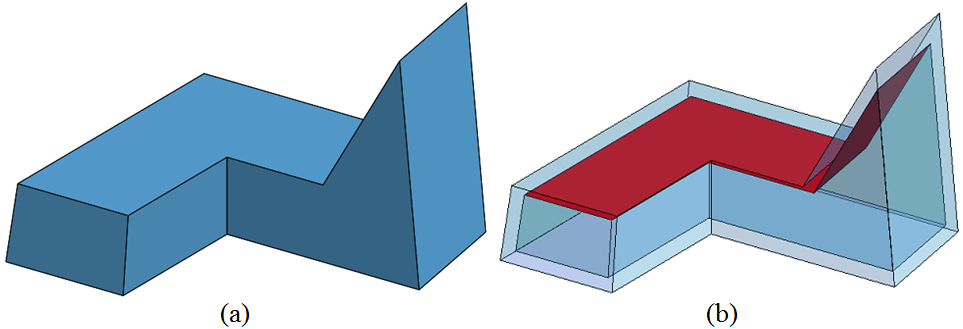
\includegraphics[width=\linewidth]{figs/solid_hollow.png}
  \caption{\label{fig:solid_hollow}%
  (a) A solid pyramid used in \cite{Hu_siga14}, and (b) a shell version of the model. The former can be printed in a support-free manner, while roof of the latter needs support.}
\end{figure}

\begin{figure*}[t]
  \centering
  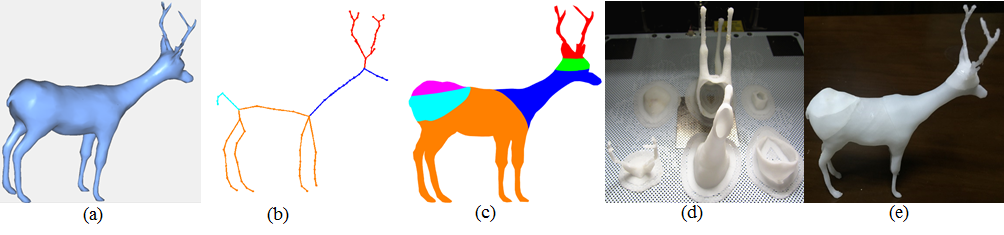
\includegraphics[width=\linewidth]{figs/tree_with_skeleton.png}
  \caption{\label{fig:ex1}%
  A deer model is partitioned into support-free parts using our algorithm: (a) a boundary mesh model; (b) skeleton partition by our approach; (c)mesh partition by our approach; (d)the support-free printing of the parts; (e) the assembly result of the printed parts.}
\end{figure*}


This paper addresses the problem of decomposing a 3{D} boundary-represented mesh, or \emph{{shell}} model which we call, into the least number of parts, each of which, when printed in a proper direction, is free of support materials. {Finding such optimum partition directly on the surface mesh is challenging as the number of mesh triangles are typically large ($10\sim100k$) and any searching algorithm could quickly lead to expediential space, demanding more effective means. We simplify the problem by considering a reduced representation. In particular,} we draw inspiration from the 1{D} skeleton of organic models: the topology variations of a natural model can be well-represented by its skeleton, and a \youyi{segment} of the skeleton corresponds to a mesh part. Further, the mesh part is typically a cylinder-like shape which can be printed free of support structures if the printing direction is parallel to the skeletal direction (Figure \ref{fig:ex1}).

We restrict our focus on \youyi{articulated or organic models whose shapes} merit well-defined skeletons. {{For a shell model}}, support structures are required for both the interior and exterior surface of a mesh model during the 3{D} printing process. Our approach assumes that the interior of a mesh model is hollow and the mesh model is shelled with a printer-friendly thickness. Therefore, our objective is to partition a model according to the growth of its skeleton into a set of parts, such that each part is represented by a skeletal subgraph and can be fabricated in a good printing direction without using any support structure. %In the meanwhile, we also look for the best partition which induces the minimal cutting length.


Formally, given a printing direction, if the angle between a facet and the printing direction is less than or equal to $\theta$ which is a printer-dependent value, then the facet can be printed without using any support structure. This inspires us to compute a minimum set of subgraph of the skeleton, such that each edge in any subgraph subtends to an axis by an angle of no larger than $\theta$, the corresponding chunk of the mesh is therefore support-free as printed along this axis (see Figure \ref{fig:fork}). %In general, a cone of axes satisfies this angle constraint.

%However, the volume of the chunk should be within the working space of the printer. Further, if the center of mass of the chunk diverts from the support center too much, e.g., the gravitational torque applied at the mass center is too far away from the center of support that it bends the printing model by a layer of thickness, then the surface quality of the model is poor or the printing task fails since the next printing layer cannot be firmly attached to the previous layer.

\youyi{Decomposing a skeleton graph into minimal set of subgraphs that satisfy the support-free constraints is a non-trivial task. In this paper, we first rigorously show that the partition problem is NP-hard by reducing a known NPC problem to it and we also show that the optimal solution can be found in polynomial time in \youyi{common} cases. Then, we present a unified stochastic framework to address the aforementioned issues by simultaneously looking for} the best set of subgraphs that are both support-free and having minimal partition length while matching a set of fabrication constraints. In short, our method makes the following contributions:

\youyi{
\begin{itemize}
\item {We devise a practical solution to the problem of support-free mesh partition by formulating it as graph partition problem with constraints;}
\item {We show the graph partition problem with support-free constraints is NP-hard;}
\item {We offer a viable and very efficient solution to tackle the graph partition problem using a semi-greedy stochastic algorithm;}
\item{We preserve the aesthetics of the surface with the least number of seams whose length is minimized.}
\end{itemize}
}
